\documentclass[a4]{report}

\usepackage{minted}
\usepackage{graphicx}
\usepackage[dvipsnames]{xcolor}
\usepackage[localise]{xepersian}

\colorlet{LightGray}{Gray!30!}
\settextfont[
  Path=fonts/,
  UprightFont = *-Regular,
  BoldFont = *-Bold,
  ItalicFont = *-Variable
]{Vazir}

\begin{document}
دانشکده مهندسی کامپیوتر و فناوری اطلاعات
\عنوان{گزارش کارآموزی\\شرکت ایده گزین روماک (اسنپ)}

\نام استاد کارآموزی{دکتر سید احمد جوادی}
\نویسنده{الهه داستان}
\شماره دانشجویی{۹۶۳۱۰۲۵}
\تاریخ{تابستان ۱۴۰۰}

\عنوان‌ساز




\فصل{چکیده}
هدف اصلي انجام این دوره کارآموزی، آشنایي و کسب تجربه‌های لازم برای ادامه کار حرفه‌ای به
عنوان یک مهندس نرم‌افزار است.

این دوره با تمرکز بر بک‌اند و در شرکت ایده گزین ارتباطات روماک (اسنپ) انجام شده است.
این دوره ابتدا با یک پروژه فردی به جهت آشنایي با تکنولوژی‌های به کار رفته و همین طور فرهنگ
سازماني شروع شد و سپس با نزدیک شدن به پایان دوره کارآموزی مشارکت در پروژه‌های اصلي شرکت انجام گرفت.

واژههای کلیدی: مهندسي نرم‌افزار، بک‌اند، سرور، تاکسي اینترنتي، حمل و نقل اینترنتي

\فصل{مقدمه}
در معماری یک نرم‌افزار، بین سخت‌افزار و کاربر لایه‌های مختلفی وجود دارد. به لایه‌هایی از این معماری که
وظیفه نمایش یک دید انتزاعی به کاربر را دارد و کاربر از طریق تعامل با آن با نرم‌افزار کار میکند بخش فرانت‌اند
میگویند. همچنین به بخشهایی که از دید کاربر پنهانند ولی در اصل منطق برنامه را شکل میدهند بخش بک‌اند
میگویند. به طور معمول بخش فرانت‌اند در بخش کاربر و بخش بک‌اند در سمت میزبان اجرا میشود.
 وجود تعداد زیادی از کاربران در محصولات بزرگ ایجاب میکند تا برنامه‌های سمت بک‌اند عالوه بر کارکرد
صحیح، به کارا‌ترین شکل ممکن نوشته شوند تا بتوانند حجمی بزرگی از درخواست را پاسخ دهند. همچنین
برنامه‌های نوشته شده باید تست‌پذیر، مستند و با خوانایی بالا باشند تا نگهداری از آن ها ساده باشد.
این گزارش به بررسی دوره کارآموزی مهندسی نرم‌افزار (بک‌اند) که در شرکت اسنپ و در تابستان ۱۴۰۰ طی شده می‌پردازد

زبان برنامه‌نویسی اصلی استفاده شده در این دوره، زبان گو بود و علاوه بر آن مهارت‌هایی نظیر کار تیمی، نوشتن کد تست‌پذیر و همچنین کار با تکنولوژی‌هایی نظیر کوبرنتیس، داکر و ... آموخته و تمرین شد.

در ادامه ابتدا به معرفی و بررسی محل کارآموزی پرداخته خواهد شد. سپس در مورد فعالیت‌ها و تجربیاتی که
در این دوره حاصل شد، توضیح داده خواهد شد و در انتها به بررسی نتایج پرداخته خواهد شد. همچنین در پایان
مراجع استفاده شده معرفی خواهند شد.

\فصل{معرفی محل کار‌آموزی}
 تاریخچه تاکسی‌های اینترنتی در ایران به سال ۱۳۹۳ و برنامه تاکسی‌یاب برمی گردد. این شرکت ابتدا با
تعداد محدودی از راننده در شهر تهران کارش را شروع کرد و سپس به اسنپ تغییر نام داد. با گذشت زمان، اسنپ
که متعلق به گروه اینترنت ایران است، به شهرهای دیگر ایران وارد شد و در این مدت مورد انتقاد صنف تاکسیرانی
قرار گرفت و به به هم زدن بازار و سفرهای ناایمن متهم شد. با این وجود اسنپ با رشد تصاعدی و کسب مقبولیت
بالا از سوی کاربران توانست به یکی از بازیگران اصلی صحنه تکنولوژی و حمل و نقل ایران بدل شود. در طی این
سالها و پیشرفت این شرکت، شرکتهای دیگری نیز به گروه اینترنت ایران پیوستند که از آن جمله میتوان به
اسنپ‌فود (سفارش غذا)، اسنپ‌مارکت (سوپرمارکت)، اسنپ‌تریپ (هتل و بلیط هواپیما) و با شیوع اپیدمی کرونا اسنپ دکتر و اسنپ داروخانه اشاره کرد.
 در تاکسی‌های اینترنتی نظیر اسنپ، کاربر با مشخص کردن مبدا، مقصد و گزینه‌هایی نظیر تاخیر در سوار
شدن، درخواست سفر میدهد. این درخواست به راننده‌های اطراف نقطه مبدا نشان داده شده و هر کدام از آنها
که سفر را قبول کنند مسئولیت جابه‌جایی مسافر را بر عهده خواهند داشت. همچنین بخش حمل کالای اسنپ
نیز همانند بخش حمل مسافر عمل میکند که اسنپ باکس نام دارد.
 بخش فنی اسنپ از تیم‌های متعددی نظیر تیم‌های بک‌اند، فرانت‌اند و دوآپس
 تشکیل شده است. در حال حاظر بخش بک‌اند اسنپ به دو تیم کوچکتر به نامهای آلفا و براوو تقسیم شده است که هر کدام بر روی پروژه‌های مختلفی کار میکنند. زبان مورد استفاده در این پروژه‌ها به طور معمول پی‌اچ‌پی و گو است
روش کار تیم‌های بک‌اند در اسنپ به صورت اسکرام است و جلسات روزانه و برنامه‌ریزی برای پیش بردن پروژه‌ها انجام میشود.
 این دوره کارآموزی در قسمت بک‌اند و در تیم براوو انجام شده است. هدف کلی پروژه‌های این تیم، بازنویسی
قسمت‌های حاضر و همچنین نوشتن امکانات جدید به زبان گو است. این دوره در ۳۰ روز و هر روز ۸ ساعت انجام
شده است.

\فصل{تکنولوژی‌های فراگرفته شده در کارآموزی}
\قسمت{نتس}
\قسمت{داکر}
 قدم بعد از توسعه نرم‌افزار این است که تصمیم گرفته شود نرم‌افزار چگونه اجرا شود. برای این که نرم‌افزارها بر روی یک میزبان به صورت ایزوله اجرا شوند یک راه سنتی این است که به ازای هر برنامه یک ماشین مجازی
بر روی میزبان بالا بیاوریم. این راه حل گرچه مشکل ایزوله بودن برنامه‌ها را حل میکند اما مشکلات بزرگی دارد.
یکی از بزرگترین مشکل‌ها این است که ماشین‌های مجازی حجم بسیاری اشغال میکنند. اجرا کردن چند ماشین
مجازی کنار هم کارایی را به شدت کاهش میدهد. همچنین زمان بالا آمدن یک ماشین مجازی زیاد است. در کنار این مشکلات، ماشین‌های مجازی مشکلاتی نظیر قابل حمل بودن نرم‌افزار، به روز‌رسانی آسان و یک‌دستی و تحویل مداوم را حل نمی‌کنند.

این مشکلات باعث شد تا احساس نیاز به یک روش جدیدتر که این مشکلات را حل کند ایجاد شود. این روش جدید کانتینرسازی نام دارد. کانتینرسازی نیز یک نوع مجازی‌سازی است که سطح مجازی‌سازی را به سطح سیستم‌عامل می‌آورد. در ماشین‌های مجازی سطح مجازی‌سازی در سطح سخت‌افزار قرار داشت.

 کانتینرها سیستم عامل مختص به خود ندارند و از سیستم عامل میزبان استفاده میکنند. به همین دلیل
کتابخانه‌ها و منابع مورد نیاز به اشتراک گذاشته می‌شوند. در کانتینرها اجرای برنامه‌ها بسیار سریع است چرا که
فایل‌های اجرایی و کتابخانه ها در هسته سیستم‌عامل میزبان اجرا میشوند

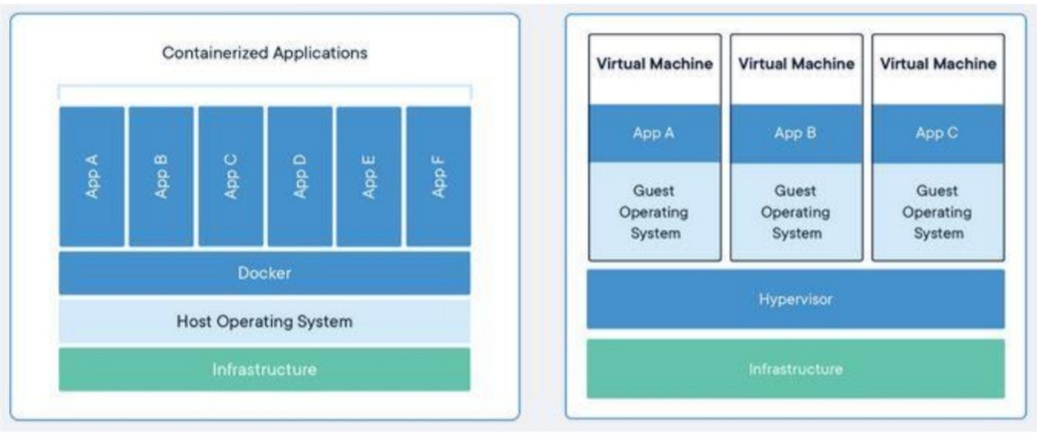
\includegraphics[scale=0.5]{fig/vm}

 داکر یک پلتفرم نرم‌افزاری است که یک برنامه را به همراه تمام نیازمندی‌های آن به فرم یک کانتینر جمع
میکند. این کار باعث میشود تا مطمئن بود برنامه در هر محیطی اجرا میشود.


\includegraphics[scale=0.5]{fig/docker}
 برای این که یک برنامه در پلتفرم داکر اجرا شود لازم است تا برای آن یک داکرفایل
نوشته شود. این فایل به صورت متن است که شامل تمام دستوراتی است که برای ساخت فایل ایمیج نیاز است. با اجرای دستور \متن‌لاتین{docker build} این ایمیج ساخته می‌شود. یک ایمیج همانند یک قالب برای ساخت کانتینر است. با اجرای دستور \متن‌لاتین{docker run} یک کانتینر از روی این قالب ساخته میشود.
 در زیر یک نمونه از داکرفایل به همراه توضیح آورده شده است.


 این دستور یک ایمیج پایه برای برنامههایی که به زبان گو نوشته شدهاند فراهم میکند.
FROM golang:1.12.0-alpine3.9
این دستور یک پوشه به نام app درست میکند.
RUN mkdir /app
این دستور محتویات ریشه را به این آدرس میبرد.
ADD . /app
این دستور به داکر اعالم میکند که از این به بعد تمام دستورات در این پوشه اجرا شوند.
WORKDIR /app
این دستور برای ساخت فایل اجرایی برنامه به زبان گو است.
RUN go build -o main .
این دستور فایل اجرایی ساخته شده را اجرا میکند.
CMD ["/app/main"]


\قسمت{کوبرنتیس}
کانتینرها راه خوبی برای ایزوله نگه داشتن برنامه در عین بالا بردن کارایی آن هستند. در مرحله اجرایی لازم است تا
کانتینر‌ها مدیریت شوند. برای مثال باید به طور دائم مواظب بود تا کانتینرها دچار خطا نشوند و در صورت وجود
خطا دوباره اجرا شوند. برای مدیریت خودکار این گونه از وظیفه‌ها میتوان از کوبرنتیس استفاده کرد.

\includegraphics[scale=0.5]{fig/kubernetes}

 کوبرنتیس یک پلتفرم متن‌باز برای مدیریت کانتینتر‌ها است. این پلتفرم در سال ۲۰۱۴ توسط گوگل متن‌باز
شد. این پلتفرم قابلیت‌های بسیاری در اختیار قرار میدهد. بعضی از این قابلیت‌ها به شرح زیر است.
1. تقسیم بار: اگر بار ورودی به یک کانتینر بیش از حد باشد، کوبرنتیس میتواند این بار را تقسیم کند
تا برنامه در حال اجرا دچار مشکل نشود.
2. مدیریت حافظه: کوبرنتیس قابلیت اختصاص بخشی از حافظه را به کانتینر‌ها میدهد.
3. مدریت منابع اجرایي: با استفاده از این قابلیت میتوان مشخص کرد چه مقدار از رم و سی‌پی‌یو برای هر کانتینر اختصاص داده شود.
4. خود‌درماني: این قابلیت باعث میشود اگر یک کانتینر دچار خطا شود و از حالت اجرا باز بماند کشته
شود و یک کانتینر مشابه از اول ساخته و جایگزین شود.

واحدی از کوبرنتیس که وظیفه مدیریت کانتینر‌ها و پیگیری این که تعداد معینی از آنها همیشه در حال اجرا باشد را دارد، دیپلویمنت نام دارد. هر دیپلویمنت شامل یک سری اطلاعات نظیر نام ایمیج داکر و تعداد کانتینری که باید اجرا شود، است. این واحد وظیفه دارد دائم در حال شمارش کانتینر‌های در حال اجرا باشد و در صورتی که این تعداد از تعداد خواسته شده کمتر باشد، یک سری کانتینر جدید بسازد و در صورتی که این تعداد از تعداد خواسته شده بیشتر باشد یک سری از آنها را بکشد.

یکی دیگر از واحدهای اصلی کوبرنتیس پاد است. پاد در واقع واحد اجرایی یک برنامه کوبرنتیس است. یک
پاد ساده‌ترین و کوچکترین واحدی است که ساخته و اجرا میشود. این واحد شامل یک یا چند کانتینر است.
در واقعیت معمولا هر پاد شامل یک کانتینر است. ذکر این نکته لازم است که کاربر به صورت مستقیم پاد‌ها را
کنترل نمیکند بلکه یک دیپلویمنت می‌سازد تا پادها را کنترل کند. یک دیپلویمنت با مدیریت یک پاد
کانتینر‌ها را کنترل میکند
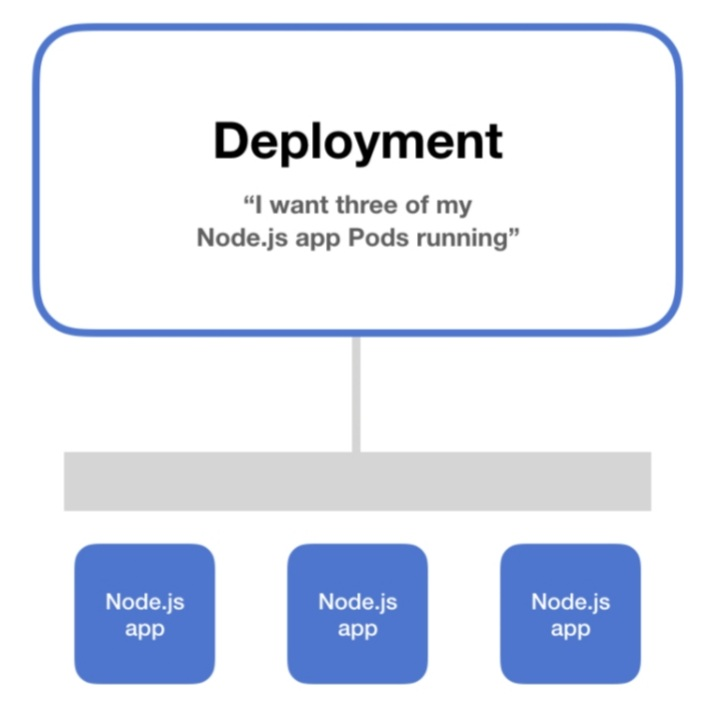
\includegraphics[scale=0.5]{fig/deployment}

برای اجرای یک برنامه در کوبرنتیس لازم است تا تنظیمات دلخواه به صورت فایل‌های یمل
بیان شوند. به عنوان مثال فایل زیر تعریف یک دیپلویمنت است که یک پاد را اجرا میکند.

apiVersion: apps/v1
kind: Deployment
metadata:
 name: test
 labels:
 app: test
spec:
 replicas: 1
 selector:
 matchLabels:
 app: test
 template:
 metadata:
 labels:
 app: test
 spec:
 containers:
 - name: test
 image: my-docker-image
 ports:
 - containerPort: 12345

 در این تنظیمات ابتدا یک دیپلویمنت با نام دلخواه ساخته شده است. این دیپلویمنت شامل یک پاد است که در فیلد رپلیکا مشخص شده است. برای این که دیپلویمنت متوجه شود کدام یک از پادها را باید مدیریت کند باید از فیلد سلکتور
 استفاده شود. در این تنظیمات برای این کار از روش پیدا کردن با اسم استفاده شده است. در نهایت فیلد مشخصات مشخص میکند که پاد باید چه کانتینری را اجرا کند.
 اگر تنظیمات فوق در فایلی به نام \متن‌لاتین{deployment.yml} ذخیره شود، کوبرنتیس میتواند آن را با دستور
زیر اجرا کند.

kubectl apply -f deployment.yml

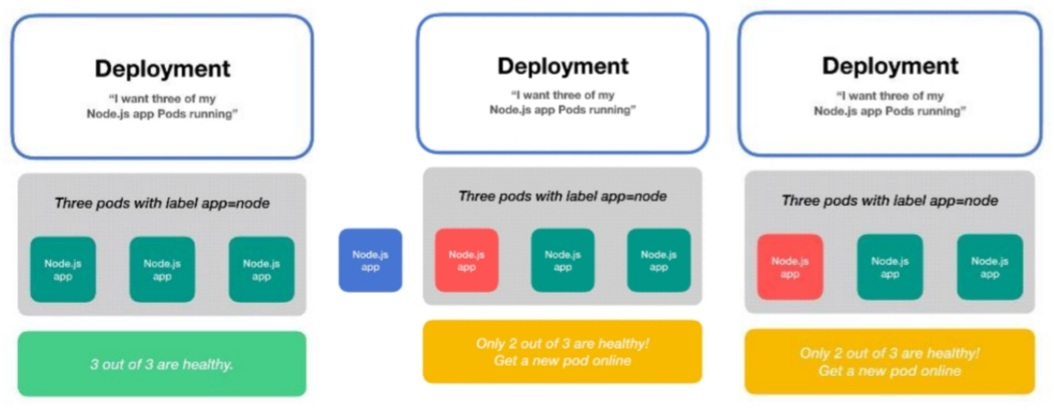
\includegraphics[scale=0.5]{fig/deploy}


حالا فرض کنید کسی بخواهد به برنامه در حال اجرا توسط کوبرنتیس از طریق شبکه متصل شود. برای این کار
میتوان آدرس آی‌پی پاد را پیدا کرد و توسط پورت برنامه به آن وصل شد. اما این روش یک مشکل بزرگ دارد. اگر پاد مثلا به دلیل خطای نرم‌افزاری یک بار خاموش و دوباره روشن شود آدرس آن عوض میشود. برای
همین باید به صورت دائم مطمئن شد که آدرس پاد به روز است. مشکل دیگر این است که ممکن است چند
نسخه از یک پاد در حال اجرا باشند. در این حالت هر کدام دارای آدرسهای مختلفی هستند و لذا هر برنامه‌ای
که بخواهد به آن متصل شود باید لیستی از آدرس‌ها را نگهداری کند.

 برای حل این مشکل کوبرنتیس دارای یک منبع به نام سرویس است. به زبان ساده یک سرویس یک آدرس ثابت در اختیار می‌گذارد که به طور خودکار به هر پادی که به آن بخورد متصل میشود. یک سرویس را میتوان همانند یک پروکسی
 تصور کرد.

 برای مثال برای تعریف یک سرویس میتوانیم به شکل زیر عمل کنیم.

 apiVersion: v1
kind: Service
metadata:
 name: my-service
spec:
 selector:
 app: test
 ports:
 - protocol: TCP
 port: 80
 targetPort: 8080

 در این تنظیمات یک سرویس ساخته شده است که پورت ۸۰۸۰ هر پادی با نام مشخص را به پورت ۸۰
بیرون متصل میکند. در این حالت برای اتصال به این سرویس کافیست از آدرس این سرویس که کوبرنتیس
به آن داده است و پورت ۸۰ استفاده کرد. اگر بیشتر از یک پاد با مشخصات خواسته شده پیدا شود، کوبرنتیس
بار را بر روی آنها تقسیم میکند.

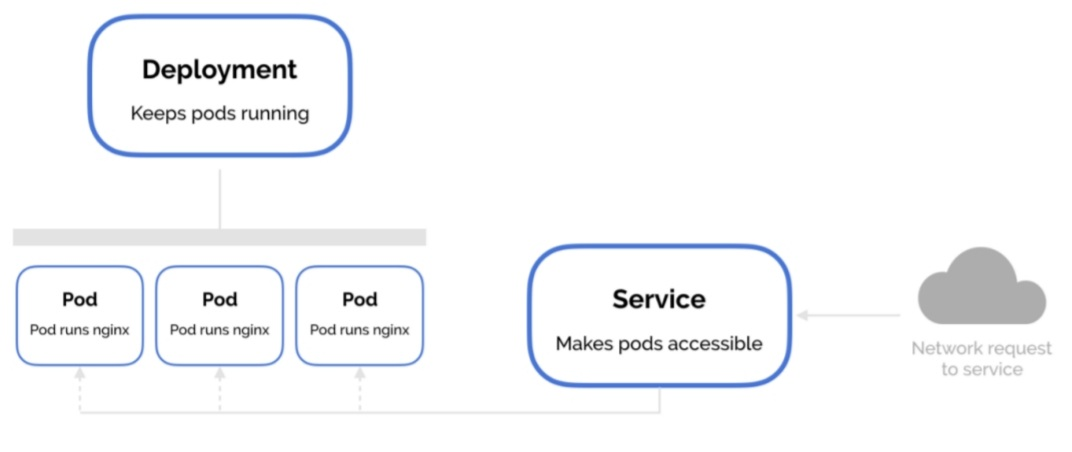
\includegraphics[scale=0.5]{fig/service}

\فصل{فعالیت‌ها و تجربیات کارآموزی}
\قسمت{هفته اول - شناخت سازمان و آشنایی با سرویس‌ها}

\پاراگراف{}
هفته‌ی اول کارآموزی بیشتر صرف شناخت ساختار شرکت و گرفتن دسترسی‌ها و خواندن کدهای قبلی می‌شود.

\پاراگراف{}
ساختار شرکت اسنپ از ساختار اسپاتیفای\پانویس{Spotify} الهام گرفته شده و حالت شطرنجی دارد.
بدین صورت که هر ونچر (منظور از ونچر بیزینس‌های مختلف می‌باشد،
به طور مثال اسنپ کب\پانویس{Snapp Cab} و اسنپ باکس\پانویس{Snapp Box} و اسنپ دکتر\پانویس{Snapp Doctor} سه ونچر متفاوت اند)
یک مدیر فنی ارشد دارد سپس هر ونچر به چندین چپتر\پانویس{Chapter} تقسیم می‌شود برای مثال در ونچر اسنپ کب که من در آن مشغول هستم
دو چپتر برای بک‌اند داریم که نام یک چپتر، آلفا\پانویس{Alpha} است که عمده سرویس‌هایشان با زبان \متن‌لاتین{PHP} توسعه یافته است و روی کد قدیمی و اولیه‌ی اسنپ کار می‌کنند.
چپتر دیگر براوو\پانویس{Bravo} است که با زبان گولنگ و روی میکروسرویس‌های جدید شرکت که از کد قدیمی جدا شده‌اند، کار می‌کند.

\پاراگراف{}
زبان گولنگ کامپایل شده، سرعت خوبی داشته و یادگیری آن ساده است. همگی این دلایل باعث شده‌اند که سرویس‌های جدید شرکت با این زبان توسعه پیدا کنند.

\پاراگراف{}
هر چپتر یک مدیر دارد که وظیفه‌ی سامان‌دهی به آن چپتر هم از نظر مدیریت افراد و هم فنی را دارد.
هر چپتر به ورتیکال‌های مختلف تفسیم می‌شود که هر ورتیکال مسئول توسعه‌ی میکروسرویس‌های مشخصی است.
هر ورتیکال نیز مدیر خود را دارد، در چپتر ما ورتیکال‌های مختلفی مانند شرد سرویسز، دیسپچیگ و … وجود دارد.

\پاراگراف{}
ورتیکالی که من در آن مشغول هستم یوزر نام دارد و تنها ورتیکالی است که به داده‌های خام کاربران دسترسی دارد و وظیفه ی ارتباط سرویس‌های داخلی
با سرویس‌های خارجی دارد مثلا ساخت اکانت و لاگین کاربران اسنپ در دست این ورتیکال است
یا ثبت نام دیجیتال راننده‌ها توسط این ورتیکال صورت میگیرد که اهمیت آن در دوران کرونا دو چندان شده است.
همچنین پنهان کردن شماره های کاربران هنگام تماس با راننده و چندین سرویس دیگر برعهده این ورتیکال است.

\پاراگراف{}
در شرکت با توجه به نیاز ورتیکال‌ها هر ورتیکال می‌تواند تعداد مختلفی نیرو در کنار نیروهای بک‌اند داشته باشد.
در ورتیکال یوزر به علت حساسیت و تنوع سرویس‌ها در کنار نیروهای بک‌اند،
نیروهای فرانت‌اند، اندروید، تست و دواپس\پانویس{DevOps} همگی حضور دارند.
با حضور نیروهای مدیریت محصول و اسکرام مستر\پانویس{Scrum} بزرگ‌ترین ورتیکال شرکت را تشکیل می‌دهد.

\پاراگراف{}
در شرکت یک نربان پیشرفت وجود دارد که هنگام ورود هر کس سطح او به او گفته می‌شود و هر ۶ ماه با توجه به عملکرد فرد که توسط مدیر ورتیکال، مدیر چپتر
و نظر سایر هم‌تیمی‌های او سنجیده می‌شود می‌تواند سطح وی ارتقا پیدا کند.

\پاراگراف{}
در شرکت از متدلوژی اسکرام استفاده می‌شود.
هر فصل در سال یک کوآرتر محسوب می‌شود که در ابتدای آن شرکت اهداف کلی را تعیین می‌کند،
که این اهداف با نظارت مستقیم مدیر فنی ارشد ونچر مشخص می‌شود.
این اهداف در اختیار ورتیکال‌ها قرار می‌گیرد و هر ورتیکال دو هفته فرصت دارد تا اهداف خود را مشخص کند به طوری که در راستای اهداف شرکت قرار بگیرد.
در ابتدای هر کوآرتر جلسات زیادی برای طراحی فنی پروژه‌ها، تخمین زمانی هر یک و \نقاط‌خ می‌شود.
هر کوآرتر به ۶ اسپیرینت\پانویس{Sprint} دو هفته‌ای تقسیم می‌شود و در ابتدای هر اسپیرینت نیز جلساتی برای انتخاب تسک‌ها و تخمین زمان آن ها تشکیل می‌شود.
در انتهای هر اسپیرینت نموداری توسط اسکرام مستر کشیده می‌شود که نشان دهنده‌ی عملکرد اعضا و عملکرد کلی تیم است
و با توجه به آن ظرفیت تیم برای اسپرینت بعدی تخمین زده می‌شود.
همچنین در انتهای هر کوآرتر اسکرام مستر با تک تک اعضا جلساتی خواهد داشت تا از دغدغه‌ها و مشکلات آن‌ها مطلع شود.
یک جلسه رترو\پانویس{Retro} نیز تشکیل خواهد شد تا هر کس نقد ها و پیشنهادات خود را برای کوآرتر بعد بیان کند و
همچنین هر کس باید به صورت ناشناس درباره ی هم تیمی هایش نظر بدهد.

\پاراگراف{}
پس از اینکه یک عضو جدید به شرکت اضافه می‌شود یک فرد از خود تیم به عنوان بادی به او معرفی می شود
که وظیفه دارد او را با تیم و سرویس‌ها آشنا کند و همچنین دسترسی‌های او را برایش فراهم کند.
هر برنامه‌نویس پس از اضافه شدن به تیم باید یک وی پی ان از شرکت بگیرد که تنها به وسیله‌ی آن می‌تواند به سرویس‌ها دسترسی داشته باشد.
همچنین باید دسترسی به ایمیل سازمانی، گیت‌لب\پانویس{Gitlab} که مخزن اصلی نگهداری کدها می‌باشد،
جیرا\پانویس{Jira} که برای مدیریت تسک‌ها می‌باشد،
کانفلوئنس\پانویس{Confluence} که برای مدیریت مستندات می‌باشد
و اسنپ کلاد\پانویس{SnappCloud} که سرویس ابری شرکت مبتنی بر \متن‌لاتین{Openshift} می‌باشد
را بگیرد.
همچنین برای آشنا شدن فرد جدید با تیم در هفته‌ی اول سعی می‌شود جلسات غیرکاری تشکیل شود که در آن اعضا بازی‌های گروهی انجام می‌دهند
و با یکدیگر آشنا می‌شوند.
همچنین فرد جدید در هفته‌ی اول باید ساختار کد‌های شرکت را مطالعه کند
و همچنین مستندات سرویس‌های ورتیکالش را مطالعه کند
تا با معماری سرویس‌های ورتیکال و شرکت آشنا شود
و بداند هر کدام از سوریس‌های تیم با چه سرویس‌هایی از سایر ورتیکال‌ها در ارتباط است.

\قسمت{هفته دوم - نشت حافظه}

\پاراگراف{}
پس از اینکه با سرویس‌های شرکت به طور کلی آشنا شدم حال باید روی یک سرویس شروع به توسعه می‌کردم.
سرویسی که برای شروع انتخاب شد سرویس ستار بود که عمل پنهان کردن شماره‌های کاربران و رانندگان را انجام می‌دهد تا امنیت بیشتری برای سفر فراهم کند.
به علت قرارداد عدم افشای اطلاعات\پانویس{NDA} که با شرکت امضا شده است و حساسیت کار این ورتیکال از توضیح معماری سرویس یا کد به هر شکل و حتی ذکر نام شرکت‌های
طرف قرارداد کاملا معذورم و به اجبار به توضیحات زیر بسنده می‌کنم.

\پاراگراف{}
سرویس پنهان کردن شماره‌های تماس در شرکت یکی از پایدارترین سرویس‌های شرکت است
که برای انجام کار خود به اطلاعات راننده‌ها و مسافران نیاز دارد
به همین جهت با پایگاه‌های داده‌ای متعددی سر و کار دارد.
همچنین برای سرعت عمل بالا از \متن‌لاتین{Redis} به عنوان حافظه نهان استفاده شده است.
برای پنهان کردن شماره‌ها شرکت با فراهم کنندگان مختلفی قرارداد دارد که ما را در این امر برقراری تماس را برعهده دارند.
سرویس‌های ما نیاز به فراخوانی این فراهم‌کنندگان دارند.
همچنین ستار خود توسط سرویس‌های دیگری از ورتیکال‌های دیگر نیز فراخوانی می‌شود و از این رو سرویس ستار
کیت توسعه سرویس (SDK) نیز دارد.
به علت وابستگی بالای این سرویس به پایگاه‌های داده‌ای مختلف و علم به اینکه پایگاه‌های داده‌ای
برای زیرساخت‌های ابری مناسب نیستند، تا اکنون این سرویس روی ماشین‌های مجازی بوده که یکی از تسک‌های مهم آن بردن این سرویس بر روی ابر است.
همچنین این سرویس تا کنون برای حالت اسنپ برای دیگری فعال نبوده که یکی از تسک‌های مهم اضافه کردن این ویژگی به آن است که طبیعتا باعث
می‌شود نیاز داشته باشیم با سرویس در شرکت به نام مورفیوس که وظیفه‌ی ارسال پیامک را دارد جهت اطلاع‌رسانی شماره‌ی پنهان شده به کاربر نیز در ارتباط داشته باشیم.
اولین مشکلی که در در این سرویس وجود داشت بحث نشت حافظه آن بود.
زمانی که در سیستم مانیتورینگ به عملکرد این سرویس در یک بازه‌ی زمانی نستا بزرگ نگاه می‌کردیم قابل مشاهده بود که حافظه مصرفی این سرویس با شیب کمی همواره در حال
افزایش است.
البته این حل این مشکل اولویت شرکت نبوده چرا که اولا اگر این سرویس از کار بیافتد نهایتا شماره‌ها پنهان نخواهند شد
که این امر در عملکرد کلی شرکت خللی وارد نمی‌کند و از طرفی چندین نسخه از این کد بالا آورده شده است که هر زمان مموری مصرفی هر کدام از حد مشخصی عبور کرد
آن نسخه با توجه به تنظیمات صورت گرفته به طور خودکار راه‌اندازی مجدد خواهد شد.
تسک اول من جستجو در کد و تحقیق جهت پیدا کردن مشکل نشتی حافظه و حل آن بود.
در جهت جستجو برای حل این مشکل اقدامات زیر انجام شد.

\پاراگراف{}
کد این سرویس نسبتا زیاد است و خواندن خظ به خط آن احتمالا زمان بسیار زیادی می‌خواست بنابراین روش بهتر این بود که یک نسخه از کد را داخل محیط تستی شرکت بالا بیاورم و
سپس آن را مانیتور کنم. اگر بدون اینکه کد زیر بار باشد سایز هیپ\پانویس{Heap} مرتبا افزایش پیدا کند به احتمال زیاد باید یک گوروتین\پانویس{Goroutine} داخل کد وجود داشته باشد
که در پس زمینه همواره در حال اجرا است و مشکلی در آن وجود دارد.
البته سایز هیپ در حالتی که ریکويستی زده نمیشد افزایش پیدا نمیکرد پس مجبور شدم آن را زیر باز ببرم این کد چندین API داشت و هر یک را لود تست و به سایز مموری رجوع می‌کردم.
هر API که زیر باز قرار گرفتن آن باعث افزایش سایز مموری شود سر نخ خوبی برای پیدا کردن مشکل است.
برای لود تست کردن از کتابخانه‌ی \متن‌لاتین{bombardier}\پانویس{https://github.com/codesenberg/bombardier} و تکه کد زیر استفاده کردم.


\begin{latin}
\begin{minted}[bgcolor=LightGray]{bash}
#!/bin/bash

for i in {1..5} ; do
  for j in {1..2000};do
    curl -v -X POST -d '{"enable": true}' \
        -H 'Content-Type: application/json' \
        https://my-service.io/api/method
    sleep .5
  done
  sleep 5m
  curl -L https://my-service.io/debug/pprof/heap > heap.$i.pprof
done
\end{minted}
\end{latin}

بعد از پیدا کردن API مورد نظر شروع به خواندن کد مربوط به آن API کردم. نکته‌ی اول که باید مد نظر قرار دهیم این است که یک کانکشن باز یا هر مورد دیگری نمی تواند باعث مموری لیک شود
اگر کد دچار مموری لیک شده یعنی داریم تکه کد مخربی را داخل یک حلقه برای مدت زمان زیادی اجرا می‌کنی.م هنگام خواندن کد باید به نکات مهمی داخل گولنگ توجه کنیم از جمله

\شروع{شمارش}
\فقره رفرنس‌ها
\فقره کانتکست‌ها
\فقره کانکشن‌ها
\فقره تیکرها
\پایان{شمارش}

\پاراگراف{}
به کدی که در ادامه می‌آید دقت کنید. یک نمونه از دیتابیس ساخنه شده و به تابع داده شده است. سپس داخل تابع یک استراکت ساخته شده که نمونه دیتابیس به عنوان یک فیلد از آن استراکت قرار گرفته است.
ممکن است انتظار داشته باشیم بعد از برگشتن از تابع \متن‌لاتین{Garbage Collector} استراکت ساخته شده را از بین ببرد اما این اتفاق نمی افتد.
چرا که این استراکت به نمونه دیتابیس رفرنس دارد که نمیتواند از بین برده شود. این اتفاق زمانی می افتد که با اشاره‌گرها کار می‌کنیم.

\begin{latin}
\begin{minted}[bgcolor=LightGray]{go}
package main

import (
        "database/sql"
        "log"
)

type Struct struct {
        db *sql.DB
        // some other fields
}

func main() {
    db, err := sql.Open("driverName", "dataSourceName")
    if err != nil {
        log.Fatalf("Cannot open database dataSourceName: %s", err)
    }

    DoSomething(db)
}

func DoSomething(db *sql.DB) {
    s := Struct{db: db}
    // do something
}
\end{minted}
\end{latin}

\پاراگراف{}
فراموش نکنید که کانتکست ها را کنسل کنید.

\begin{latin}
\begin{minted}[bgcolor=LightGray]{go}
package main

import "context"

func main() {
    ctx, cancelCtx := context.WithCancel(context.Background())
    defer cancelCtx()
}
\end{minted}
\end{latin}

\پاراگراف{}
هر سوکت که باز می‌شود باید حتما بسته شود. البته اکثرا از کتابخانه‌ها برای باز کردن سوکت استفاده می‌کنیم. این کتابخانه ها خود موارد مختلفی را هندل می‌کنند تا بعد از اتمام کار ما سوکت بسته شود.
اما به هر حال باید به آن توجه کنیم چراکه حالاتی وجود دارد که سوکت باز می‌ماند به تکه کد زیر دقت کنید.

\begin{latin}
\begin{minted}[bgcolor=LightGray]{go}
package main

import (
    "database/sql"
    "log"
)

type Storage struct {
    db *sql.DB
    // some other fields
}

func (s *Storage) fetchAll() {
    // *Rows should be closed
    rows, err := s.db.Query("SELECT * FROM somewhere")
    if err != nil {
            log.Fatal(err)
    }

    defer func() {
        err := rows.Close()
        if err != nil {
                log.Fatal(err)
        }
    }()

    if err := rows.Err(); err != nil {
        log.Fatal(err)
    }

    // If Next is called and returns false and there are no
    // further result sets, the Rows are closed automatically
    // but an error may occur inside the block
    for rows.Next() {
        // If this error or any other one occurs, this loop doesn't continue
        // so if I hadn't called close in a defer function we would have an
        // open connection forever
        err := rows.Scan("&dest")
        if err != nil {
            return
        }
    }
}

func main() {
    // usually we make a single db instance and use
    // it during the whole project life,
    // so it's rare to call Close function on it
    db, err := sql.Open("driverName", "dataSourceName")
    if err != nil {
        log.Fatalf("Cannot open database dataSourceName: %s", err)
    }

    s := Storage{db: db}
    s.fetchAll()

    // some other code
}
\end{minted}
\end{latin}

\پاراگراف{}
دقت کنید که تیکرها بعد از شروع، متوقف شوند.

\begin{latin}
\begin{minted}[bgcolor=LightGray]{go}
package main

import "time"

func main() {
    ticker := time.NewTicker(time.Second)
    defer ticker.Stop()
}
\end{minted}
\end{latin}

\پاراگراف{}
مشکل کد که باعث نشتی حافظه می‌شد به دلیل ساختن تیکرها داخل حلقه و متوقف نکردن آن‌ها بود. تکه کدی مانند زیر


\begin{latin}
\begin{minted}[bgcolor=LightGray]{go}
package main

import "time"

func main() {
    go func() {
        for time.Now(); true; <-time.NewTicker(time.Second).C {
            // Do something
        }
    }()

    // Do something
}
\end{minted}
\end{latin}

\پاراگراف{}
برای آنکه مطمئن شوم نشتی حافظه به دلیل تکه کد بالا به وجود آمده است با تکه کد زیر آن را تست کردم:

\begin{latin}
\begin{minted}[bgcolor=LightGray]{go}
package main

import (
    "fmt"
    "runtime"
    "time"
)

func main() {
    // Below is an example of using our PrintMemUsage() function
    // Print our starting memory usage (should be around 0mb)
    PrintMemUsage()

    ticker := time.NewTicker(time.Millisecond)
    defer ticker.Stop()
    for time.Now(); true; <-ticker.C {
        a := 2
        a *= 2
        if a == 1024 {
            a = 2
            // Force GC to clear up, should see a memory drop
            runtime.GC()
        }
        PrintMemUsage()
    }
}

// PrintMemUsage outputs the current,
// total and OS memory being used.
// As well as the number
// of garage collection cycles completed.
func PrintMemUsage() {
    var m runtime.MemStats
    runtime.ReadMemStats(&m)

    // For info on each,
    // see: https://golang.org/pkg/runtime/#MemStats
    fmt.Printf("Alloc = %v MiB", bToMb(m.Alloc))
    fmt.Printf("\tTotalAlloc = %v MiB", bToMb(m.TotalAlloc))
    fmt.Printf("\tSys = %v MiB", bToMb(m.Sys))
    fmt.Printf("\tNumGC = %v\n", m.NumGC)
}
\end{minted}
\end{latin}

برنچی از مستر گرفتهو این تکه کد که باعث نشتی حافظه می‌شد را تغییر دادم و مرج ریکويست را قرار دادم. پس از مرور برنچ توسط مدیر ورتیکال این برنچ با مستر مرج شد.

\قسمت{هفته سوم - سفر برای دیگری}

\پاراگراف{}
در هفته‌ی سوم فرصت برای توسعه‌ی بیشتر روی سرویس ستار به وجود آمد.
در هنگام گرفتن سفر در اکانت می‌توانید مشخص کنید که این سفر را برای خوتان می‌خواهید یا برای دوستتان.
اگر سرویس پنهان کردن شماره را فعال کرده باشید و اسنپ را برای خودتان بخواهید هیچ مشکلی نخواهید داشت اما اگر برای فرد دیگری سفر بگیرید شماره‌ها پنهان نخواهند شد.
تسک این هفته اضافه کردن این قسمت به کد بود.
با توجه به اینکه کد بسیار ماژولار بود و هر عملکرد یکتایی تابع و استراکت خود را داشت اضافه کردن این فیچر کار بدون دردسری بود.
در ابتدا تنها دو نفر داخل مساله بودند حال با اضافه کردن نفر سوم گراف ذهنی ما باید
تغییر پیدا کند.

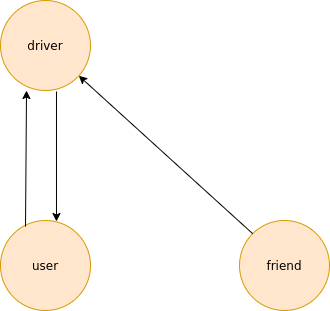
\includegraphics[scale=0.5]{fig/call-graph}

\پاراگراف{}
در گراف بالا نود دوست اضافه شده است که باید به کد نیز اضافه میشد علاوه بر آن زمانی که سفر برای دوست گرفته می‌شود و سرویس ستار فعال است
باید از طریق پیامک شماره‌ی پنهان شده‌ی راننده به فرد سوم مورد نظر اطلاع‌رسانی شود.
به همین دلیل باید با سرویس مورفیوس که وظیفه‌ی پیام رسانی را دارد نیز ارتبط می‌داشتیم.
همچنین همانطور که بیان شد سرویس ستار توسط سرویس‌های دیگری داخل شرکت صدا زده میشد که از SDK استفاده می‌کردند
به همن جهت SDK این سرویس نیز باید تغییر داده میشد و به تیم‌هایی که این سرویس را کال می کردند اطلاع رسانی میشد.


\پاراگراف{}
پس از اضافه کردن فیچر، ریویو توسط مدیر مستقیم ورتیکال و رفت و آمد برای انجام تغییرات درخواست مدیر ورتیکال، نوبت به تست آن می‌شود
چون هیچ فیچر جدید یا تغییر زیاد در کد بدون امضای نیرو کیفیت سرویس نمی‌تواند منتشر شود. برای تست کردن باید ابتدا کد را داخل محیط تستی دیپلوی می‌کردم و در ارتباط با کیفیت سرویس می‌بودم
تا اگر باگی در کد وجود داشت با مانیتور کردن لاگ‌ها هنگام تست متوجه اشکال میشدم. پس از تست کیفیت سرویس برنچ در برنچ مستر مرج می‌شود
حال برای بالا بردن این فیچر باید کد جدید روی سرورها دیپلوی شود.
دیپلوی حتما باید در نیمه شب انجام شود تا اگر به هر دلیل اگر خطایی به وجود آمد، ضرر کمتری به تجارت شرکت وارد شود. تنها مدیر مستقیم ورتیکال اجازه‌ی دیپلوی و دسترسی \متن‌لاتین{SSH} به سرورها
پروداکشن دارد علاوه بر او باید فرد دیگری که علاوه بر توسعه دهنده‌ی فیچر است حضور داشته باشند و در زمان دیپلوی به دقت سرویس را مانیتور کند و اگر تغییر غیر عادی در ترافیک سرویس‌ها
دید باید فیچر سریعا رول‌بک شود. لازم به ذکر است برخی از فیچرها که بسیار حساس باشند علاوه بر تایید مدیرمستقیم ورتیکال به تایید مدیر چپتر نیز نیاز دارند.

\پاراگراف{}
گروه‌های رسمی ای در پیام‌رسان سازمانی تشکیل می‌شوند که یکی از آن‌ها مربوط دیپلوی سرویس‌ها است. هر تیم قبل از ریلیز باید در آن گروه اعلام کند که در حال دیپلوی است و نام سرویس را ذکر کند
تا اگر مشکلی به وجود آمد تمامی افراد از جمله دواپس بدانند که ریلیزی صورت گرفته و تمامی احتمالات را در نظر بگیرند.

\قسمت{هفته چهارم - بردن سرویس به ابر}

\پاراگراف{}
در این هفته بحث بردن سرویس ستار روی ابر مطرح شد. همانطور که در گزارش هفته‌های پیش بیان کردم این سرویس به علت وابستگی به چندین پایگاه داده و
عدم کارکردن مناسب پایگاه‌های داده با ابر، این سرویس روی ماشین‌های مجازی در حال سرویس‌دهی بود، اما با توجه به سیاست‌های شرکت همه‌ی تیم‌ها سعی می‌کنند
تا تمامی سرویس‌های خود را روی ابر بالا بیاورند تا نگه‌داری آن‌ها به عهده‌ی تیم ابر اسنپ باشد و تیم‌ها خود درگیری کمتری برای نگه‌داری آن‌ها بعد از دیپلوی داشته باشند.
به همین جهت در این هفته من باید کار با \متن‌لاتین{Kubernete} و ابر را یاد می‌گرفتم.
روزهایی در هفته صرف یادگرفتن چگونگی کارکرد \متن‌لاتین{Kubernetes} و معماری پشت آن شد تا درک عمیق تری از اتفاقاتی که در پشت آن می‌افتد پیدا کنم.
همچنین باید روی سیستمی که شرکت در اختیار من گذاشته بود \متن‌لاتین{Docker} نصب می‌کردم که به علت تحریم‌ها برای نصب و استفاده از این سرویس باید پشت
چندین سرویس \متن‌لاتین{VPN} قرار می‌گرفتم که دردسرهای زیادی داشت و وقت زیادی صرف آن شد.
پس از آن باید فایل‌های \متن‌لاتین{YAML}ای می‌نوشتم که به وسیله‌ی آن ها سرویس روی ابر دیپلوی می‌شود که در واقع به آن‌ها \متن‌لاتین{manifest}های سرویس گفته می‌شود.
البته استفاده از \متن‌لاتین{Helm Chart} به جای دستی نوشتن فایل‌های \متن‌لاتین{manifest} کار توسعه و نگهداری را بسیار راحت‌تر می کرد اما ورتیکال یوزر هنوز به آن روی نیاورده و باید فایل‌های
\متن‌لاتین{manifest} دستی نوشته شوند.

\پاراگراف{}
\متن‌لاتین{Kubernetes} دارای \متن‌لاتین{manifest}های متنوعی است که می‌بایست با توجه به نوع سرویس از آن‌ها استفاده شود.
این \متن‌لاتین{manifest}ها در جهت توصیف \متن‌لاتین{pod} که کوچکترین عنصر در محیط \متن‌لاتین{Kubernetes} بوده و خود از چند \متن‌لاتین{container}
تشکیل شده است تا عناصر بزرگی مانند \متن‌لاتین{Deployment} و \نقاط‌خ استفاده می‌شوند.

\پاراگراف{}
در سرویس ستار ما از \متن‌لاتین{Deployment} استفاده کردیم چرا که نمونه‌های مختلف ستار به یکدیگر وابسته نبوده و می‌توانند مستقل فعالیت کنند.
به این ترتیب مدیریت آن‌ها کامل به \متن‌لاتین{Kubernetes} سپرده می‌شود تا در صورت خرابی یا افزایش لود و \نقاط‌خ تعداد \متن‌لاتین{pod}ها را افزایش یا کاهش دهد.
برای آشنایی بیشتر شایان ذکر است که \متن‌لاتین{Deployment} در واقع مدیریت \متن‌لاتین{pod}ها را بر عهده می‌گیرد و آن‌ها افزایش یا کاهش می‌دهد.
در ضمن سلامت آن‌ها را نیز مطابق با آنچه در \متن‌لاتین{manifest} بیان شده است مانیتور می‌کند.

\پاراگراف{}
برای دسترسی به سرویس‌ها می‌بایست پورت‌های آن‌ها در قالب یک \متن‌لاتین{manifest} تعریف شود. این \متن‌لاتین{manifest} \متن‌لاتین{Service} نام دارد.
برای سرویس ستار نیز یک \متن‌لاتین{Service} تعریف شده و پورت‌های آن تعریف گشت.

\پاراگراف{}
هر پروژه نیازمنده تنظیمات است و این تنظیمات در قالب \متن‌لاتین{mainfest}های \متن‌لاتین{ConfigMap} و \متن‌لاتین{Secret} تعریف می‌شوند.
در نظر داشته باشید که تنظیمات شما چه طریق فایل و چه طریق متغیرهای محیطی تعریف شده باشند این \متن‌لاتین{manifest}ها برای شما مورد نیاز خواهند بود.

\پاراگراف{}
دست آخر ستار می‌بایست توسط سایر سرویس‌های شرکت که ممکن است روی ابر باشند یا نباشند مورد فراخوانی قرار می‌گیرد. از این روی برای آن یک \متن‌لاتین{manifest}
به نام \متن‌لاتین{Route} تعریف می‌شود. که اجازه تعریف \متن‌لاتین{URL} برای دسترسی به سرویس را می‌دهد.
این \متن‌لاتین{URL}ها خود می‌توانند به صورت \متن‌لاتین{Public} و \متن‌لاتین{Private} باشند.

\پاراگراف{}
در نهایت من این فایل‌ها را حاضر کردم و بنابر استاندارد تیم فایل اسکریپتی برای نصب همزمان همه این \متن‌لاتین{manifest}ها روی ابر نوشتم.
این کار روی ابر تستی تیم تست شده و در نهایت آماده برای اجرای روی پروداکشن شد.

\قسمت{هفته پنجم - نوشتن مستندات}
\پاراگراف{}
در این هفته وارد پروژه ی دیگری می‌شوم که بقیه‌ی اعضای تیم نیز روی آن کار می‌کنند.
این پروژه در جهت تسهیل ثبت‌نام رانندگان توسعه داده می‌شود تا قبل از همه گیری کرونا رانندگان برای ثبت نام به صورت حضوری به شعبه‌هایی می‌رفتند و ثبت نام خود را انجام می‌دادند.
پس از کرونا این شعبه ها باید بسته می‌شدند همچنین رانندگان نیز میلی به ثبت نام حضوری نداشتند و از همان موقع پروزه‌ی ثبت‌نام دیجیتالی رانندگان در اولویت شرکت قرار گرفت این پروژه باید در اسرع وقت منتشر می‌شد
به همین علت در دست تیم دیگری قرار گرفته بود و با زبان \متن‌لاتین{PHP} و در چهارچوب \متن‌لاتین{Wordpress} توسعه داده شده بود.
حتی پس از آن نیز یک نسخه جدیدتری از آن توسط تیم دیگری توسعه داده شده بود و حال باید نسخه سوم توسط تیم ما توسعه یابد تا این فرایند کامل دیجیتال شود و کل فرآیند ثبت نام به کوتاه‌ترین زمان ممکن برسد.
همچنین بحث حفظ اطلاعات کاربران وامنیت آن‌ها ارتقا یابد و این اطلاعات تنها در دست تیم ما باشد.
این هفته جلسه‌های بسیاری با نیروهای محصول تیم و همچنین چندین جلسه‌ی طراحی سیستم تشکیل شد. دو مساله‌ی برجسته در این پروژه وجود داشت اول ماشین حالت\پانویس{State Machine} پروژه دوم مشکل نشت اطلاعات کاربران

\پاراگراف{}
این پروژه تمامی اعضای بک‌اند، فرانت‌اند، اندروید، مدیریت پایگاه داده، تیم ابر و طراحی را درگیر می‌کند. اغلب ورتیکال یوزر خود پایگاه داده‌ای‌ خود را نگه‌داری می‌کند اما در این پروژه نگه‌داری دیتابیس در دست تیم مدیریت پایگاه داده است.

\پاراگراف{}
وقتی یک راننده می‌خواهد ثبت نام کند ابتدا توسط پروژه‌ی دیگری که باز هم در دست تیم ما است احراز هویت می شود.
اگر احراز هویت موفقیت آمیز بود سرآیندی در درخواست کاربر تنظیم می‌شود و این درخواست به سمت پروژه‌ی \متن‌لاتین{Driver Signup} می‌آید.
جهت اینکه احراز هویت برای کاربران راحت‌تر باشد و پیگیری اطلاعات از طریق سازمان‌های مرتبط نیز راحت‌تر صورت گیرد، از کاربران خواسته می‌شود عکس مدارک خود مانند گواهینامه، کارت‌ماشین، بیمه و غیره را گرفته و آپلود کنند.
این عکس‌ها در \متن‌لاتین{minio} دخیره می‌شوند اما با این حال باید اطلاعات کاربر در پایگاه‌داده‌ای نیز دخیره شود در نتیجه نیاز به تبدیل کردن عکس مدارک به متن است که توسط شرکت دیگری انجام می شود.
پس از اینکه از نظر سیستم مشکلی وجود نداشت مثلا راننده‌ای که قصد ثبت نام دارد قبلا راننده‌ای نبوده که بلاک شده است یا مسائلی از این قبیل،
این مدارک و متن آن‌ها در داشبردی در دست نیروی انسانی قرار می‌گیرد تا هم متن مدارک چک شود و اگر خطایی وجود دارد اصلاح شود و همچنین مدارک به طور کلی بار دیگر چک شوند تا از صحت آنان اطمینان یابیم.

\پاراگراف{}
در این هفته جلسه‌ی مروری برگزار شد و یکی از مشکلات اعضای تیم روند کند بررسی شدن کدها بود به همین دلیل از این هفته دیگر نیازی نیست تا کد تنها توسط مدیر تیم بررسی شود
و هر کس پس از توسعه‌ی برنچ خود کافی است تایید تنها یک عضو دیگر را بگیرد و برنچ مرج می شود اما برنچ ها باید همگی به دستی تست شوند.

\پاراگراف{}
از آن جایی که اعضای فرانت و بک‌اند همکاری زیادی باهم در این پروژه خواهند داشت نوشتن مستندات و به روز نگه داشتن آن اهمیت بسیاری دارد
و می‌تواند از تداخل‌های زیادی جلوگیری کند. اولین تسک من نوشتن \متن‌لاتین{swagger}، براساس صحبت‌ها و تصمیم‌گیری‌های انجام شده در جلسه‌ی طراحی راه‌حل بود.
پروژه دارای رابط‌های برنامه‌نویسی زیر است:

\شروع{فقرات}
\فقره فرستادن رمز یکبار مصرف به راننده
\فقره تایید رمز یکبار مصرف
\فقره آپلود عکس مدارک راننده
\فقره متقاضی راننده شدنر
\پایان{فقرات}

البته این رابط‌های برنامه‌نویسی به خارج از شرکت ارائه می‌شوند، علاوه بر آنها رابط‌های زیر برای داخل شرکت می‌باشند:

\شروع{فقرات}
\فقره گرفتن تسک‌ها برای افراد مرور کننده
\فقره گرفتن افراد متقاضی
\فقره گرفتن افراد ارجاع‌دهنده
\پایان{فقرات}

آخرین رابط کاربری لیست افراد ارجاع‌دهنده را بر می‌گرداند. ارجاع‌دهنده‌ها افرادی هستند که می‌توانند یک راننده را ثبت‌نام کنند و از آن جایی که استخدام خود شرکت هستند
می‌توانند، خود شخصا راننده را احراز هویت کنند و در نتیجه راننده‌هایی که از طریق ارجاع‌دهنده‌ها ثبت‌نام می‌شوند حالتی متفاوت در ماشین حالت ذکر شده دارند.

\پاراگراف{}
در این هفته این \متن‌لاتین{swagger} نوشته و مرج شد.

\فصل{نتیجه‌گیری}
در این دوره کارآموزی با تکنولوژیهای روز دنیا در توسعه نرمافزار بکاند آشنایی حاصل شد. اولین تکنولوژی
معرفی شده در این دوره آپاچی کافکا بود که یک پلتفرم انتقال داده انعطافپذیر است و در صورت استفاده درست
از آن، میتواند با کارایی باال در جابهجایی اطالعات کمک کند. این پلتفرم دارای کتابخانههای زیادی برا زبانهای
مختلف برنامهنویسی است. از آن جا که زبان استفاده شده در این دوره زبان گو بود الزم بود تا از کتابخانه ساراما
که مربوط به این زبان است استفاده شود.
 برای این که یک برنامه در محیط واقعی به کارکرد صحیح ادامه دهد باید تستهای مختلفی روی آن انجام شده
است. این تست قطعات کوچک برنامه 46 باشد. یکی از این تستها که توسعهدهنده میتواند انجام دهد، تست واحد
)نظیر توابع( را از نظر درستی کار بررسی میکند. برای این که برنامه بتواند مورد تست واحد قرار بگیرد، باید
تستپذیر باشد. این نکته به این معنی است که توسعهدهنده باید با ذهنیتی برنامه را بنویسد که قابل تست باشد.
در این دوره کارآموزی سعی شد که این نکته رعایت شود.
 برای اجرای برنامه در محیط میزبان راهی که در پروژههای شخصی انجام میشد اجرای برنامههای مختلف در
کنار هم در یک سیستم عامل بود. این روش اگر چه برای پروژههای شخصی سرراست و آسان است ولی در
محیطهای تجاری و بزرگتر مشکلساز میشود. یکی از این مشکالت این است که برنامهها به راحتی به هم و
منابع هم دیگر دسترسی دارند . مشکل دیگر این است که منابع سیستم عامل بین برنامهها مشترک است و هر
کدام میتوانند به تمامی منابع دسترسی داشته باشند. برای حل این مشکل، قبلتر، از ساخت ماشین مجازی برای
هر برنامه استفاده میشد. این روش گرچه مشکالت قبلی را ندارد ولی سربار حجم و زمان آن بسیار باال است و
کارایی خوبی ندارد. روش مدرنتری که استفاده میشود روش کانتینرسازی است. این روش برای هر برنامه یک
ماشین مجازی مجزا باال نمیآورد و همه برنامهها از منابع سیستم عامل میزبان استفاده میکنند ولی هر برنامه
برای خود دارای یک محیط ایزوله است. برای اجرای یک برنامه در کانتینر از داکر استفاده شد. برای مدیریت این
کانتینرها در زمان اجرا و جلوگیری از خاموش شدن آنها به علت خطای نرمافزاری از پلتفرم کوبرنتیس استفاده
شد.
 یکی از راههای بهبود پروژه اصلی انجام شده این دوره کارآموزی این است که کد آن با هدف افزایش قابلیت
تست واحد بازنویسی شود.

کوبرنتیس یک پلتفرم گسترده و پیچیده است که در این دوره کارآموزی فقط از قابلیتهای پایهای آن استفاده
شد. یک راه بهبود استفاده از آن این است که قابلیتهای پیشرفتهتر آن در پروژههای دیگر استفاده شوند. این کار
عالوه بر این که به یادگیری آن کمک میکند، در کارایی باالتر نرمافزارهای اجرا شده با آن نیز تاثیر دارد.
\end{document}
